\documentclass[conference]{IEEEtran}
\IEEEoverridecommandlockouts
% The preceding line is only needed to identify funding in the first footnote. If that is unneeded, please comment it out.
\usepackage{cite}
\usepackage{amsmath,amssymb,amsfonts}
\usepackage{algorithmic}
\usepackage{graphicx}
\usepackage{textcomp}
\usepackage{xcolor}
\usepackage{svg}
\usepackage{hyperref}
\svgpath{{./images/}}
\def\BibTeX{{\rm B\kern-.05em{\sc i\kern-.025em b}\kern-.08em
    T\kern-.1667em\lower.7ex\hbox{E}\kern-.125emX}}
\begin{document}

\title{VisioMel Challenge: Predicting Melanoma Relapse\\
% {\footnotesize \textsuperscript{*}Note: Sub-titles are not captured in Xplore and
% should not be used}
% \thanks{Identify applicable funding agency here. If none, delete this.}
}

\author{\IEEEauthorblockN{1\textsuperscript{st} Mahadev Prasad Panda}
\IEEEauthorblockA{\textit{M.Sc. Artificial Intelligence} \\
\textit{Friedrich-Alexander-Universität Erlangen-Nürnberg (FAU)}\\
Erlangen, Germany \\
mahadev.prasad.panda@fau.de}
}
\maketitle
\begin{abstract}
Relapse assessment is an important part of melanoma diagnosis and treatment. 
% Recent advances in machine learning and deep learning have shown tremendous promise in a variety of medical applications.
In this study, we investigated several approaches for predicting melanoma recurrence using digital microscopic slides and clinical metadata. We conducted experiments using one machine learning strategy and four deep learning approaches, indicating that deep learning models outperform machine learning models in terms of predictive performance. Notably, our work employs a two-stage strategy, with the first stage including image-only training, followed by a second stage involving fine-tuning utilizing the features of images from the first stage and the addition of clinical metadata to improve predictive power of the deep learning models. Additionally, we further enhanced the predictive capacity of our models by transforming Whole Slide Images (WSIs) into stitched tiles. Overall, our findings demonstrate that deep learning methods, particularly with two-stage training strategy and tile stitching, can improve relapse prediction.
\end{abstract}

\begin{IEEEkeywords}
Melanoma Relapse Prediction, Deep Learning, Machine Learning, Two-Stage Strategy, Stitched Tiles
\end{IEEEkeywords}

\section{Introduction}
Melanoma, an aggressive kind of skin cancer caused by melanocytes, is a major worldwide health problem, with a high number of annual diagnosis and fatalities \cite{b1}.
More often than not the fatalities are caused by a recurrence of the disease after the successful initial diagnosis and treatment. So, effective melanoma prognosis and therapy are crucially dependent on properly estimating the likelihood of relapse, which necessitates a detailed assessment of the tumor's microscopic characteristics as well as the patient's clinical history. Currently, this is mostly the duty of skilled pathologists who meticulously examine tissue samples under a microscope. Despite their unrivaled knowledge, the burgeoning fields of deep learning and machine learning provide a great chance to improve their diagnostic abilities and perhaps revolutionize melanoma recurrence prediction.

More than 325,000 melanoma cases were recorded in 2020, resulting in nearly 57,000 deaths globally and it is expected by the year 2040 the total number of cases and deaths due to melanoma is expected double in numbers \cite{b1}. Melanoma accounts for approximately 22\% of all skin malignancies and is known for its capacity to spread, making it critical to properly and quickly estimate the risk of relapse in order to develop customized treatment methods for each patient \cite{b1}. 

% \begin{figure}[h!]
%   \centering
%   \includesvg[inkscapelatex=false, width = 200pt]{melanoma_projection.svg}
%   \caption{Melanoma cases and deaths in year 2020 and predicted cases and deaths for year 2040.}
%   \label{fig:melanoma_projection}
% \end{figure}

Recent developments in machine learning and deep learning, notably in the area of histopathological image interpretation, have shown enormous promise in a variety of medical applications. Deep learning methods have shown capability of performing fundamental tasks like measuring an area on Whole Slide Image (WSI) and have even shown potential when it comes to categorising different tumour subtypes \cite{b2, b3, b4}. In terms of melanoma recurrence prediction, the combination of these cutting-edge technologies with the knowledge of pathologists offers up new avenues with the possibility of improved accuracy, effectiveness, and accessibility in clinical settings.

This technical report offers a thorough investigation that uses machine learning and deep learning methods to create a prediction model for melanoma recurrence in the first five years of initial diagnosis, by databases of histopathology images along with pertinent clinical information as shown in Figure \ref{fig:aim}. We investigate the viability of automating the risk assessment process, hence allowing early identification and individualised treatment approaches. To mitigate difficulties with melanoma recurrence prevention, our recommended approach can be used independently or to supplement the diagnostic skills of a pathologist.
\begin{figure}[h!]
  \centering
    \includesvg[inkscapelatex=false, width = 200pt]{aim.svg}
  \caption{Schematic diagram of overall relapse prediction process.}
  \label{fig:aim}
\end{figure}
% Keeping the aim of predicting relapse in mind, we investigate the following research problems through our experimentation. 
% \begin{itemize}
%     \item 
% \end{itemize}

\section{Data Set}

\subsection{Data Description}
The dataset consists Whole Slide Images (WSI), clinical metadata and labels.

\subsubsection{Whole Slide Images (WSI)}
Whole Slide Images (WSIs) are digitized versions of traditional microscopic glass slides commonly used in pathology. WSIs are provided in the pyramidal TIF format, which is a tiled, multi-resolution structure. The TIF file contains multiple layers or "pages," with Page 0 representing the WSI at its full resolution. Each successive page is a downsampled version of the previous one, reducing the image size by a factor of two. This pyramidal arrangement enables quick access to various magnification levels, facilitating efficient examination of specific areas of interest in the WSI.

\begin{figure}[h!]
  \centering
    \includesvg[width = 150pt]{slide.svg}
  \caption{Example of a WSI with annotations. Among the annotations the yellow line shows Breslow and orange area shows Ulceration.}
  \label{fig:slide}
\end{figure}

An example of WSI is shown in the figure \ref{fig:slide} with different annotations.  In this image, the yellow line represents Breslow, indicating the thickness of the melanoma in millimeters. Additionally, the orange area on the figure corresponds to Ulceration, signifying the total loss of epidermal tissue.

\subsubsection{Clinical Metadata}
The metadata includes clinical information such as filename, age, sex, body site, melanoma history, breslow, and ulceration, which were collected from patients during their initial diagnosis. Each patient is associated with a pyramidal TIF image, and each row in the metadata CSV file corresponds to a unique patient. The filename column serves as a distinct identifier that links the images to their corresponding clinical data. Breslow column contains melanoma thickness in mm and ulceration column shows whether ulceration is present in melanoma or not. Breslow and ulceration are two important indicators which pathologist focus on to predict likelihood of relapse. 
\subsubsection{Labels}
Labels for this dataset come from patients' medical records which indicate whether the patient was diagnosed with a melanoma relapse in the 5 years after initial diagnosis. Lables file contain two columns filename and relapse. Filename is the unique identifier for each patient which is same as the filename column in the clinical metadata. The relapse column is a binary column where 0 represents no relapse and 1 represents relapse.

\subsection{Exploratory Data Analysis}
\subsubsection{Data distribution over relapse}
\begin{figure}[h!]
  \centering
    \includesvg[width = 200pt]{relapse_norelapse.svg}
  \caption{Data distribution over relapse.}
  \label{fig:relapse}
\end{figure}
Figure \ref{fig:relapse} shows the data distribution over relapse. The dataset exhibits a significant class imbalance. Among the 1342 observations, only 213 observations pertain to positive relapse cases, while a substantial majority of 1129 observations correspond to no relapse cases. It is crucial to address this imbalanced distribution during model training to avoid bias towards the dominant class. Failure to account for this imbalance could lead the model to favor predictions for the majority class, potentially compromising its performance on detecting positive relapse cases.

\subsubsection{Data distribution over Breslow}
\begin{figure}[h!]
  \centering
    \includesvg[width = 200pt]{breslow.svg}
  \caption{Data distribution over Breslow.}
  \label{fig:breslow}
\end{figure}

Figure \ref{fig:breslow} shows the data distribution over Breslow. The percentage of relapse cases shows an upward trend with increasing Breslow width. The lowest percentage of relapse cases is observed for Breslow widths less than 0.8 mm, whereas for Breslow widths greater than 4 mm, the number of relapse cases exceeds that of non-relapse cases. This shows Breslow is an important indicator for prediction of relapse.
\subsubsection{Data distribution over ulceration}
\begin{figure}[h!]
  \centering
    \includesvg[width = 200pt]{ulceration.svg}
  \caption{Data distribution over ulceration.}
  \label{fig:ulceration}
\end{figure}

Figure \ref{fig:ulceration} shows the data distribution over ulceration.  The presence of ulceration significantly influences the percentage of relapse cases, with the percentage being notably low for cases without ulceration. In contrast, the number of relapse cases increases substantially when ulceration is present. This shows ulceration is an important indicator for prediction of relapse.

\section{Methodologies}
With Breslow and ulceration being crucial indicators for relapse prediction, their absence in the test set due to the need for expert pathologist annotations poses a challenge. To address this, our model is designed to learn these concepts implicitly without directly using Breslow and ulceration as input. Instead we use these features as additional targets of our model along with relapse turning the problem into a multitask learning approach. Our methodologies and experiments aim to answer two research questions:

\textbf{Training Approach}: We investigate whether it is more effective to train the model with metadata and WSIs together in a single stage or separately in two stages.

\textbf{Handling WSI Size}: Given the large size of WSIs, we explore whether utilizing lower resolutions or extracting patches from higher resolution WSIs is more suitable for training the models effectively.

To achieve these aims, we implemented the following methods: 

\begin{itemize}
    \item Whole slide model (Deep Learning model using both WSI and meta data)
    \begin{itemize}
        \item Single Stage
        \item Two Stage
    \end{itemize}
    \item Patch based model (Deep Learning model using patches from WSI and meta data)
    \begin{itemize}
        \item Single Stage
        \item Two Stage
    \end{itemize} 
    \item Base model (Machine Learning only using meta data)
\end{itemize}


\subsection{Whole Slide Model}

Firstly, we employed a single-stage deep learning approach as shown in the figure \ref{fig:single_stage_wsi}  using the ResNet-34 \cite{b5} model as our image feature extractor. The output of this model is passed through a series of fully connected layers and is combined with the processed meta-data using another set of fully connected layers. The resulting concatenated output is then fed through an additional set of fully connected layers. The final output of these layers is fed into three classification layers, where we perform classification for Breslow, ulceration, and relapse.

Throughout the fully connected layers, we utilized ReLU as the activation function and applied a dropout rate of 0.2 to prevent overfitting. To address the issue of class imbalance, particularly for relapse, we adopted Focal loss \cite{b6}. For Breslow, we used cross-entropy (CE) loss, and for ulceration, we employed binary cross-entropy (BCE) loss. 

Additionally, we implemented a two stage variant of our approach. During the first stage, we exclusively trained the image feature extractor to predict relapse, relapse ulceration, and Breslow. In the second stage, we kept the image feature extractor fixed and focused on training the remaining parts of the model. The detailed model architectures can be found in Appendix 1.

In the first stage, for training, we utilized BCE loss for ulceration and relapse predictions and CE loss for Breslow prediction. During the second stage, we employed Focal loss for relapse, BCE loss for ulceration, and CE loss for Breslow prediction. 
% This two-stage approach allowed us to enhance the performance and adapt the model effectively to handle different aspects of the task
\begin{figure}[h!]
  \centering
    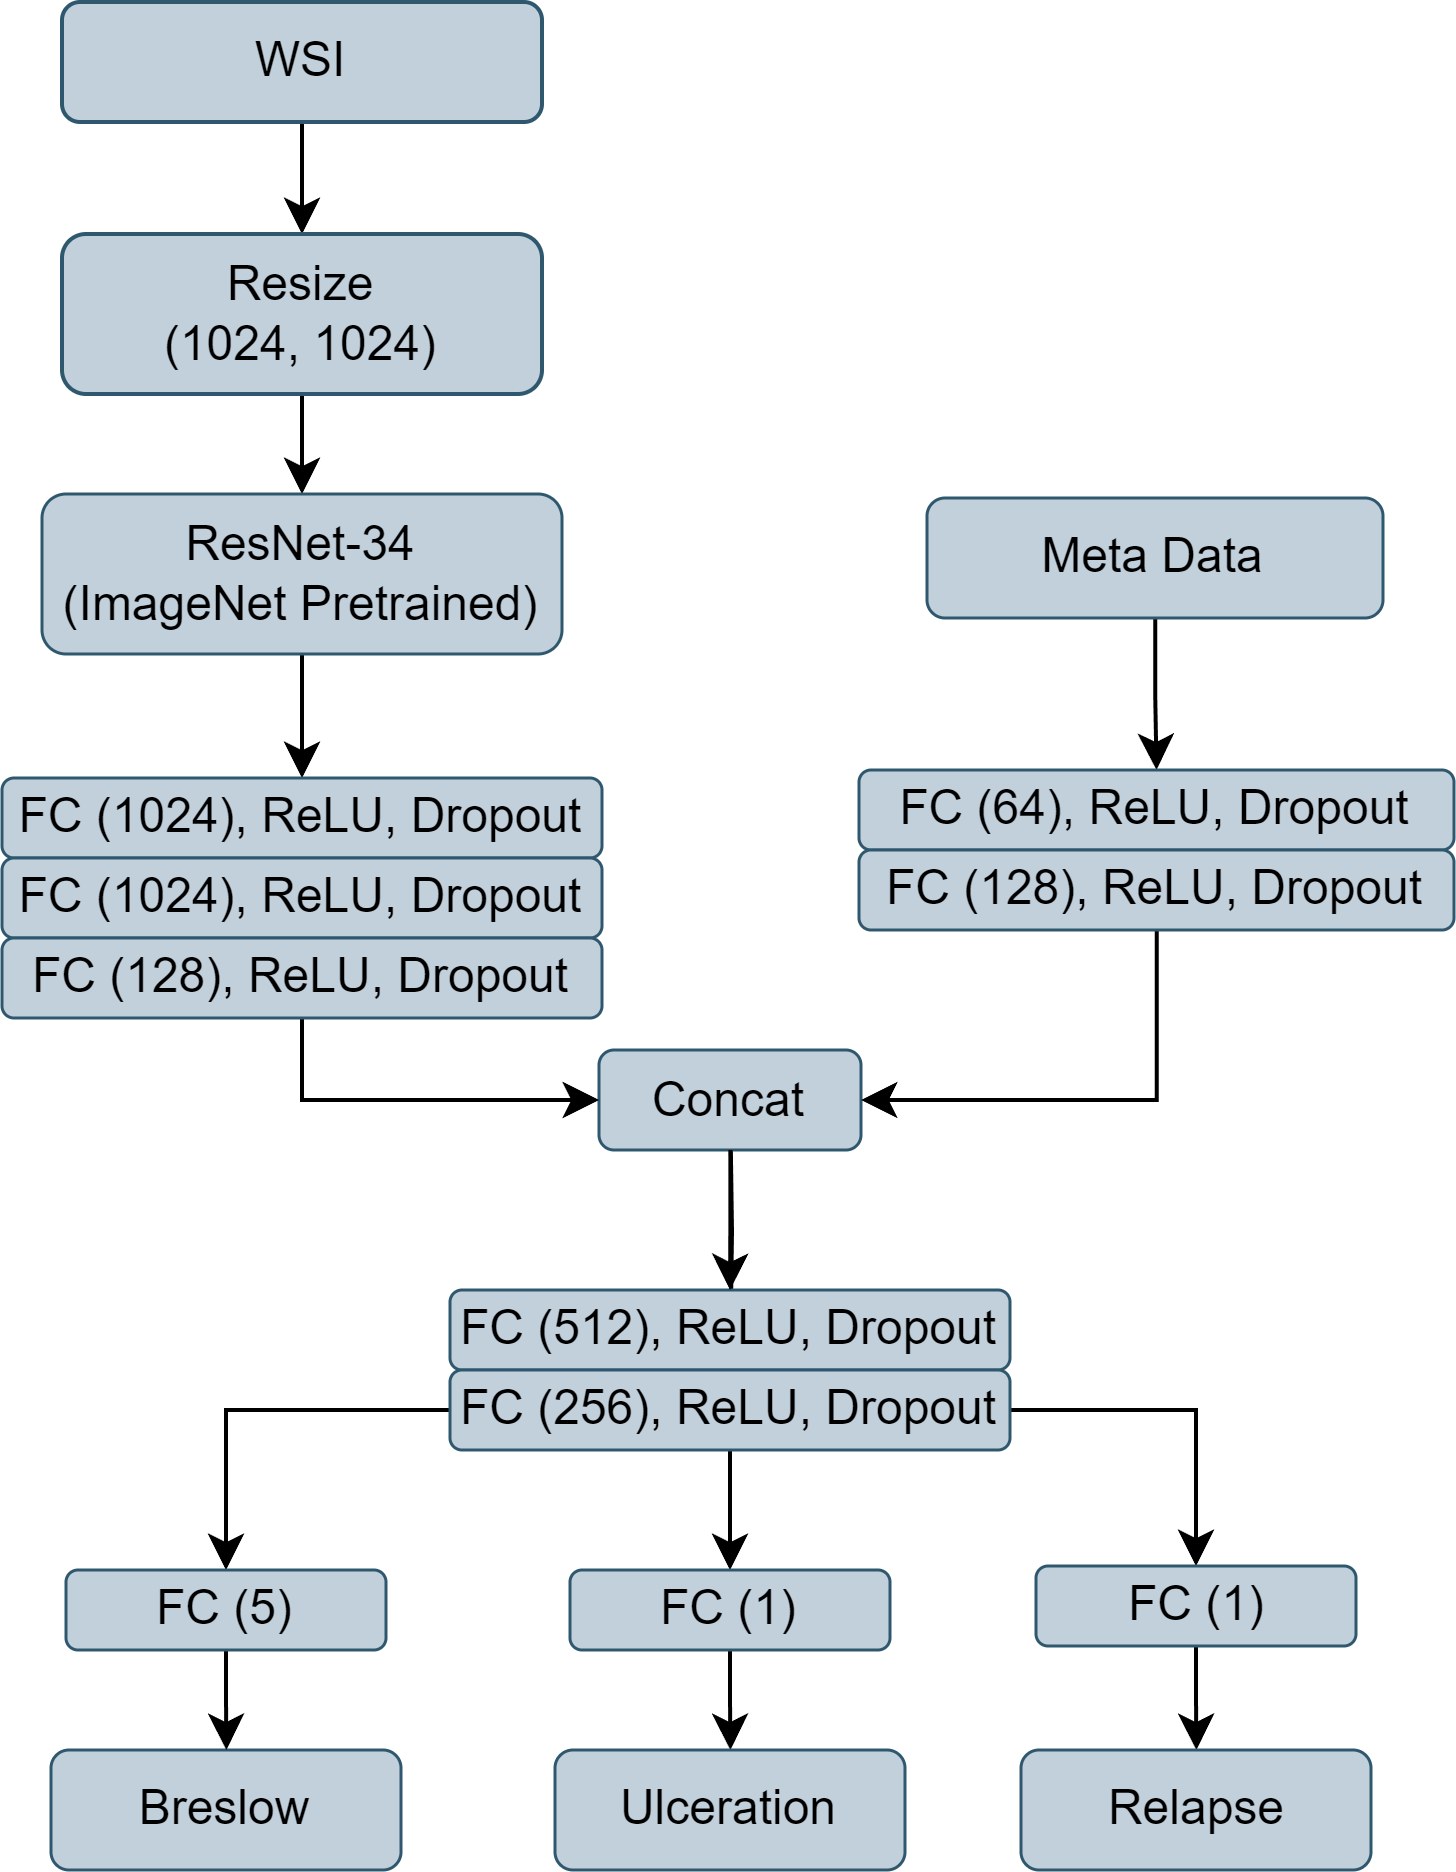
\includegraphics[scale=0.15]{images/page0.png}
  \caption{Whole Slide Model Single stage approach.}
  \label{fig:single_stage_wsi}
\end{figure}
\subsection{Patch Based Model}
The second method we utilized in our study is the patch-based model. In this approach, we leveraged the observation that whole-slide images (WSI) often contain significant white background regions, while the tissue areas are relatively sparse. To capitalize on this characteristic, we devised a tiling procedure, which we refer to as ``tiling" in our work, as depicted in Figure \ref{fig:tiling}.

\begin{figure}[h!]
  \centering
    \includesvg[inkscapelatex=false, width = 200pt]{Tilling.svg}
  \caption{Schematic diagram of the tiling procedure.}
  \label{fig:tiling}
\end{figure}

The first step in the tiling process involves the extraction of a binary tissue mask from the RGB whole-slide image (WSI). To achieve this, we convert the RGB image into the HED color space and apply a threshold to the E channel, which allows us to obtain the tissue mask. By multiplying this mask with the original WSI, we create a masked WSI that focuses solely on the tissue regions of interest.

Next, we divide the masked WSI into non-overlapping tiles of size 256x256. During this process, any tiles that do not contain any tissues are discarded, ensuring that we only retain relevant regions for further analysis. Among the tissue-containing tiles, we select the top 36 tiles based on their intensity levels, which helps us to capture significant features while managing computational complexity.

To efficiently process the selected tiles, we concatenate them into a single image, referred to as the "stitched image." This stitched image serves as the input to our deep learning model, replacing the original high-resolution WSI. By adopting this tiling approach, we achieve notable improvements in computational efficiency and memory requirements, as we focus on processing the smaller stitched image rather than the entire high-resolution WSI. 

We implemented single stage and two stage variant of this approach which are exactly the same as the whole slide model single stage and two stage variants with additional tiling step. The exact architecture of these approaches are shown in the Appendix 1.

\subsection{Base Model}
Finally we implemented a machine learning approach that works only on the metadata. As Breslow and ulceration are not available for test data we removed these columns from training set. We used an AutoML frame work called AutoGluon \cite{b7} to predict relapse by taking age, sex, body site and melanoma history as input.



\section{Experimental Setup \& Results }
During the training process, we divided the dataset into training (64\%), validation (16\%), and test sets (20\%). For all methods, we employed the Adam optimizer with a batch size of 16 and an initial learning rate of 1e-4. To schedule the learning rate, we used Reduce on Plateau. In the single-stage approach, the models were trained for 100 epochs, while the two-stage approach consisted of training the first stage for 50 epochs and the second stage for another 50 epochs. To determine the optimal epoch, we selected the point where the model performed best on the validation set. Throughout the training, we employed the loss function specified in equation \ref{eq:loss} to optimize the models' performance for Breslow, ulceration, and relapse predictions. $\lambda$ represents the weighting factor for loss of Breslow and ulceration. 

\begin{equation}
        \mathcal{L} = \mathcal{L}_{relapse} + \lambda * \left( \mathcal{L}_{breslow} + \mathcal{L}_{ulceration}\right)
        \label{eq:loss}
\end{equation}

\begin{table}[htbp]
\caption{Comparison of all model performance on different metrics on the test set.}
\centering
\begin{tabular}{|l|l|l|l|l|l|}
\hline
Metrics       & \begin{tabular}[c]{@{}l@{}}Base \\ Model\end{tabular} & \begin{tabular}[c]{@{}l@{}}Single \\ Stage \\ WSI \\ Model\end{tabular} & \begin{tabular}[c]{@{}l@{}}Two \\ Stage \\ WSI \\ Model\end{tabular} & \begin{tabular}[c]{@{}l@{}}Single \\ Stage \\ Stitched \\ Model\end{tabular} & \begin{tabular}[c]{@{}l@{}}Two \\ Stage \\ Stitched \\ Model\end{tabular} \\ \hline
Accuracy (↑)  & 0.74                                                  & 0.71                                                                    & 0.74                                                                 & 0.8                                                                          & 0.76                                                                      \\ \hline
Recall   (↑)  & 0.55                                                  & 0.7                                                                     & 0.76                                                                 & 0.76                                                                         & 0.77                                                                      \\ \hline
Precision (↑) & 0.54                                                  & 0.62                                                                    & 0.66                                                                 & 0.68                                                                         & 0.67                                                                      \\ \hline
F1 Score (↑)  & 0.55                                                  & 0.62                                                                    & 0.66                                                                 & 0.7                                                                          & 0.68                                                                      \\ \hline
ROC\_AUC (↑)  & 0.6                                                   & 0.79                                                                    & 0.82                                                                 & 0.81                                                                         & 0.81                                                                      \\ \hline
TNR (↑)       & 0.82                                                  & 0.72                                                                    & 0.73                                                                 & 0.81                                                                         & 0.76                                                                      \\ \hline
TPR   (↑)     & 0.28                                                  & 0.67                                                                    & 0.79                                                                 & 0.7                                                                          & 0.79                                                                      \\ \hline
FNR   (↓)     & 0.72                                                  & 0.33                                                                    & 0.21                                                                 & 0.3                                                                          & 0.21                                                                      \\ \hline
FPR (↓)       & 0.18                                                  & 0.28                                                                    & 0.27                                                                 & 0.19                                                                         & 0.24                                                                      \\ \hline
\end{tabular}

\label{tab:results}
\end{table}

Following model training, an extensive evaluation was conducted on the test dataset using a range of performance metrics, including accuracy, recall, precision, F1-score, area under the ROC curve, true negative rate, true positive rate, false positive rate, and false negative rate. The outcomes of these evaluations are presented in Table \ref{tab:results}. It was observed that the deep learning models outperformed the machine learning model. This can be attributed to the utilization of both clinical metadata and whole slide images (WSIs) by the deep learning models, while the machine learning model relied solely on clinical metadata. Additionally, the increased complexity of the deep learning models compared to the machine learning models likely contributed to their superior performance.

As delineated in Table \ref{tab:results}, the two-stage models exhibited a slightly enhanced performance in comparison to the single-stage model. This improvement is postulated to stem from the specialized training of the image feature extractor for the classification of Breslow, ulceration, and relapse. This dedicated training likely facilitated the extraction of more pertinent features from the WSIs. Similarly, the models employing a stitching strategy displayed slightly better performance than those without it. This phenomenon can be elucidated by the fact that stitching leverages higher resolution images for patch extraction, whereas WSI-based models employ lower resolution WSIs due to inherent complexity limitations.

\section{Conclusion and Future Work}

In this study, we assessed five approaches (one machine learning, four deep learning) for relapse prediction. Deep learning methods outperformed the machine learning approach, with the patch based model two stage variant  showing slight superior performance in metrics like Recall, True Positive Rate, and False Negative Rate. The two-stage and stitched tile strategies improved models' performance. Future enhancements could stem from hyper-parameter optimization, refined segmentation models, and more advanced stitching techniques (structure preserving rather than in the order of intensity). In conclusion, our findings highlight deep learning methods' efficacy, particularly with two-stage and stitched tile strategies, and suggest potential avenues for further research to enhance relapse prediction.


\begin{thebibliography}{00}
\bibitem{b1} Arnold M, Singh D, Laversanne M, et al. Global Burden of Cutaneous Melanoma in 2020 and Projections to 2040. JAMA Dermatol. 2022;158(5):495–503. doi:10.1001/jamadermatol.2022.0160
\bibitem{b2} Comes, M., Fucci, L., Mele, F. et al. A deep learning model based on whole slide images to predict disease-free survival in cutaneous melanoma patients. Sci Rep 12, 20366 (2022). https://doi.org/10.1038/s41598-022-24315-1
\bibitem{b3} Nicolas Loménie, Capucine Bertrand, Rutger H.J. Fick, Saima Ben Hadj, Brice Tayart, Cyprien Tilmant, Isabelle Farré, Soufiane Z. Azdad, Samy Dahmani, Gilles Dequen, Ming Feng, Kele Xu, Zimu Li, Sophie Prevot, Christine Bergeron, Guillaume Bataillon, Mojgan Devouassoux-Shisheboran, Claire Glaser, Agathe Delaune, Séverine Valmary-Degano, Philippe Bertheau,
Can AI predict epithelial lesion categories via automated analysis of cervical biopsies: The TissueNet challenge?, Journal of Pathology Informatics, Volume 13, 2022, 100149, ISSN 2153-3539,
https://doi.org/10.1016/j.jpi.2022.100149.
\bibitem{b4} Soong SJ, Ding S, Coit D, Balch CM, Gershenwald JE, Thompson JF, Gimotty P; AJCC Melanoma Task Force. Predicting survival outcome of localized melanoma: an electronic prediction tool based on the AJCC Melanoma Database. Ann Surg Oncol. 2010 Aug;17(8):2006-14. doi: 10.1245/s10434-010-1050-z. Epub 2010 Apr 9. PMID: 20379784; PMCID: PMC8635121.
\bibitem{b5} K. He, X. Zhang, S. Ren and J. Sun, "Deep Residual Learning for Image Recognition," 2016 IEEE Conference on Computer Vision and Pattern Recognition (CVPR), Las Vegas, NV, USA, 2016, pp. 770-778, doi: 10.1109/CVPR.2016.90.
\bibitem{b6} T. -Y. Lin, P. Goyal, R. Girshick, K. He and P. Dollár, "Focal Loss for Dense Object Detection," 2017 IEEE International Conference on Computer Vision (ICCV), Venice, Italy, 2017, pp. 2999-3007, doi: 10.1109/ICCV.2017.324.

\bibitem{b7} Erickson, Nick, et al. "AutoGluon-Tabular: Robust and Accurate AutoML for Structured Data." arXiv preprint arXiv:2003.06505 (2020).

\end{thebibliography}

\section{Appendix 1: Model Architectures}
\begin{figure}[h!]
  \centering
    \includegraphics[scale=0.55]{images/page1.png}
  \caption{Whole Slide Model Two Stage approach, stage one.}
  \label{fig:wsi_s1}
\end{figure}
\begin{figure}[h!]
  \centering
    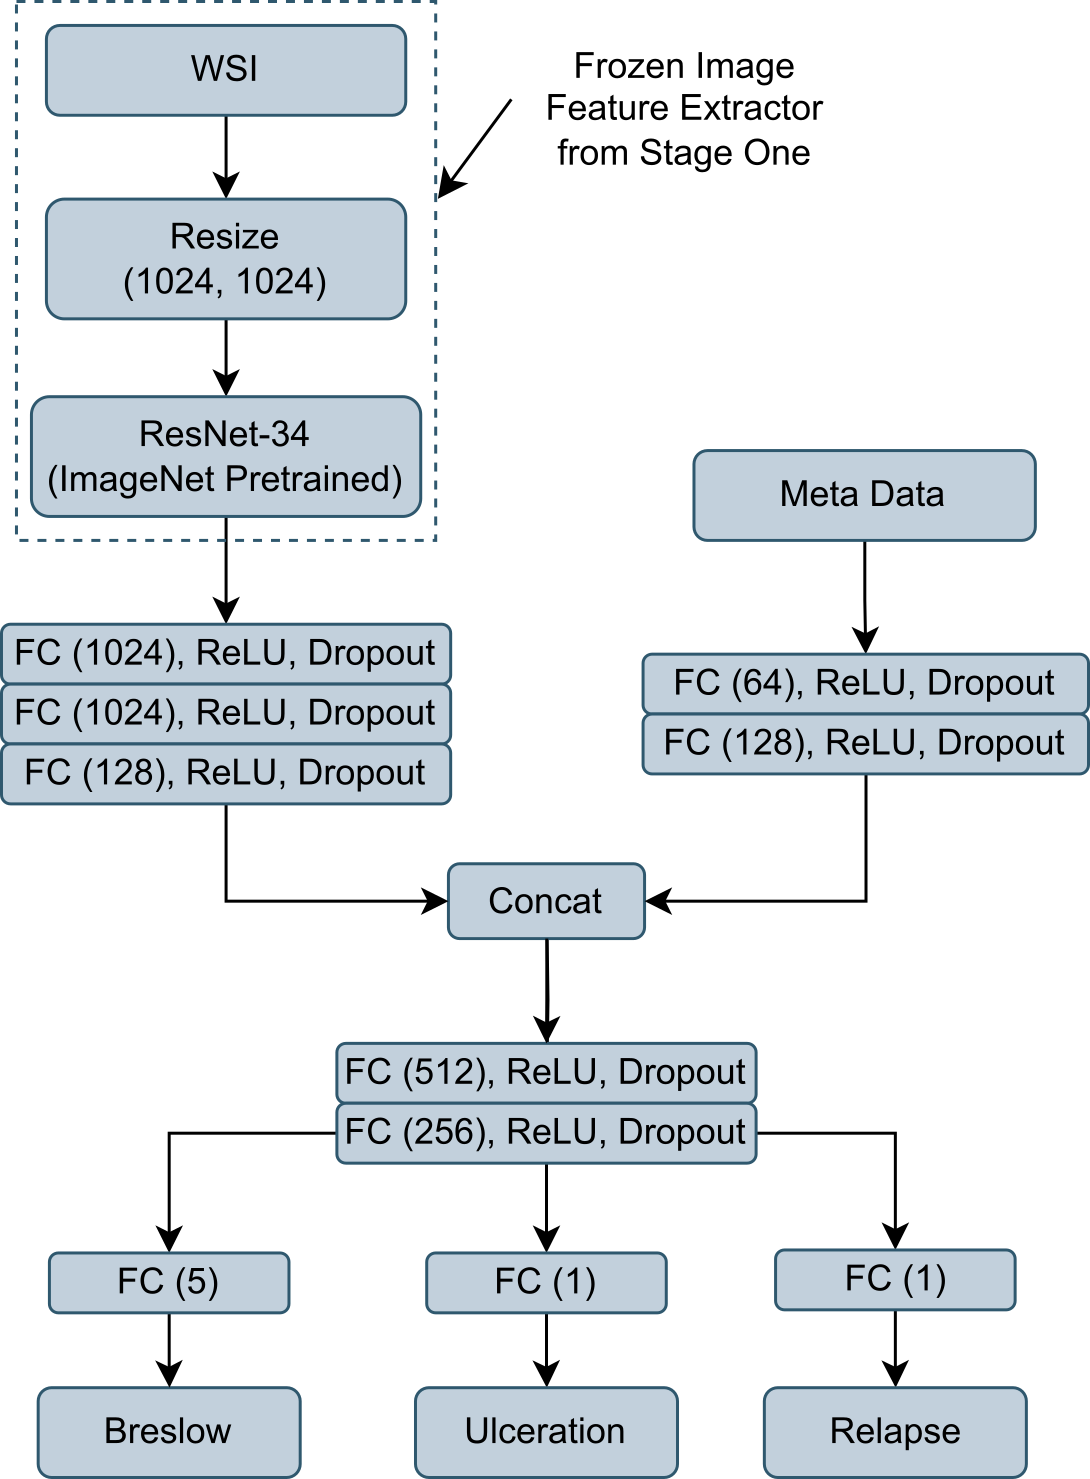
\includegraphics[scale=0.5]{images/page2.png}
  \caption{Whole Slide Model Two Stage approach, stage two.}
  \label{fig:wsi_s2}
\end{figure}
\begin{figure}[h!]
  \centering
    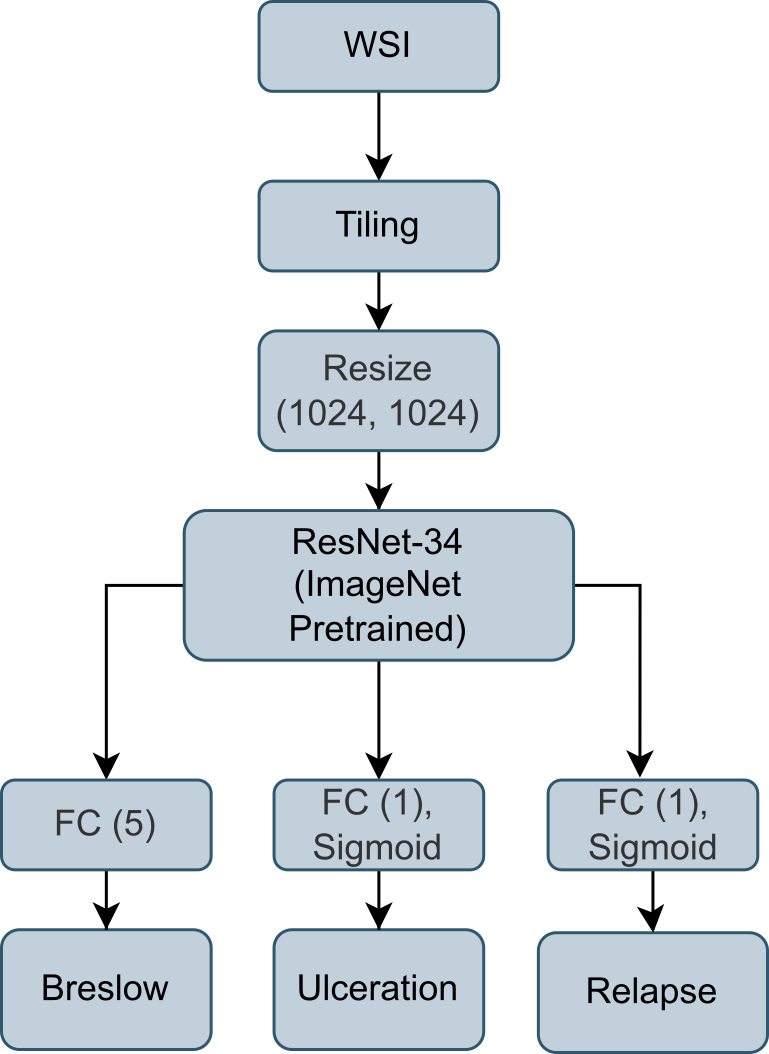
\includegraphics[scale=0.6]{images/page3.png}
  \caption{Patch Based Model Two Stage approach, stage one.}
  \label{fig:pbm_s1}
\end{figure}
\begin{figure}[h!]
  \centering
    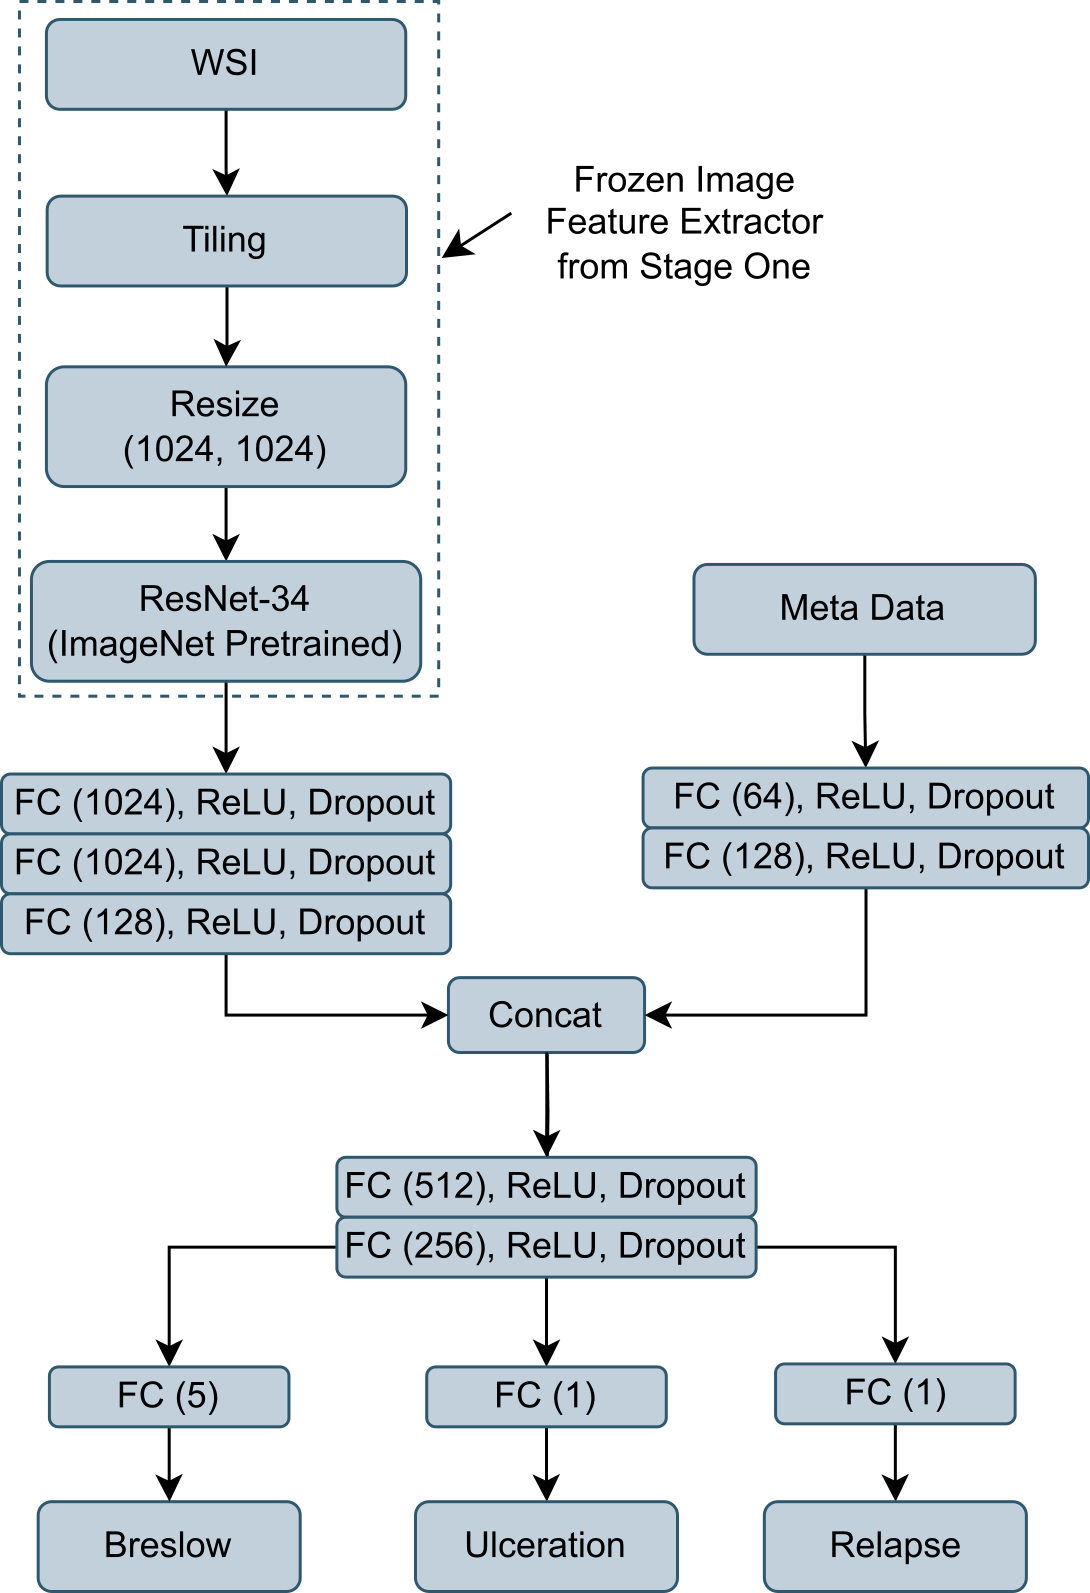
\includegraphics[scale=0.55]{images/page4.png}
  \caption{Patch Based Model Two Stage approach, stage two.}
  \label{fig:pbm_s2}
\end{figure}
\begin{figure}[h!]
  \centering
    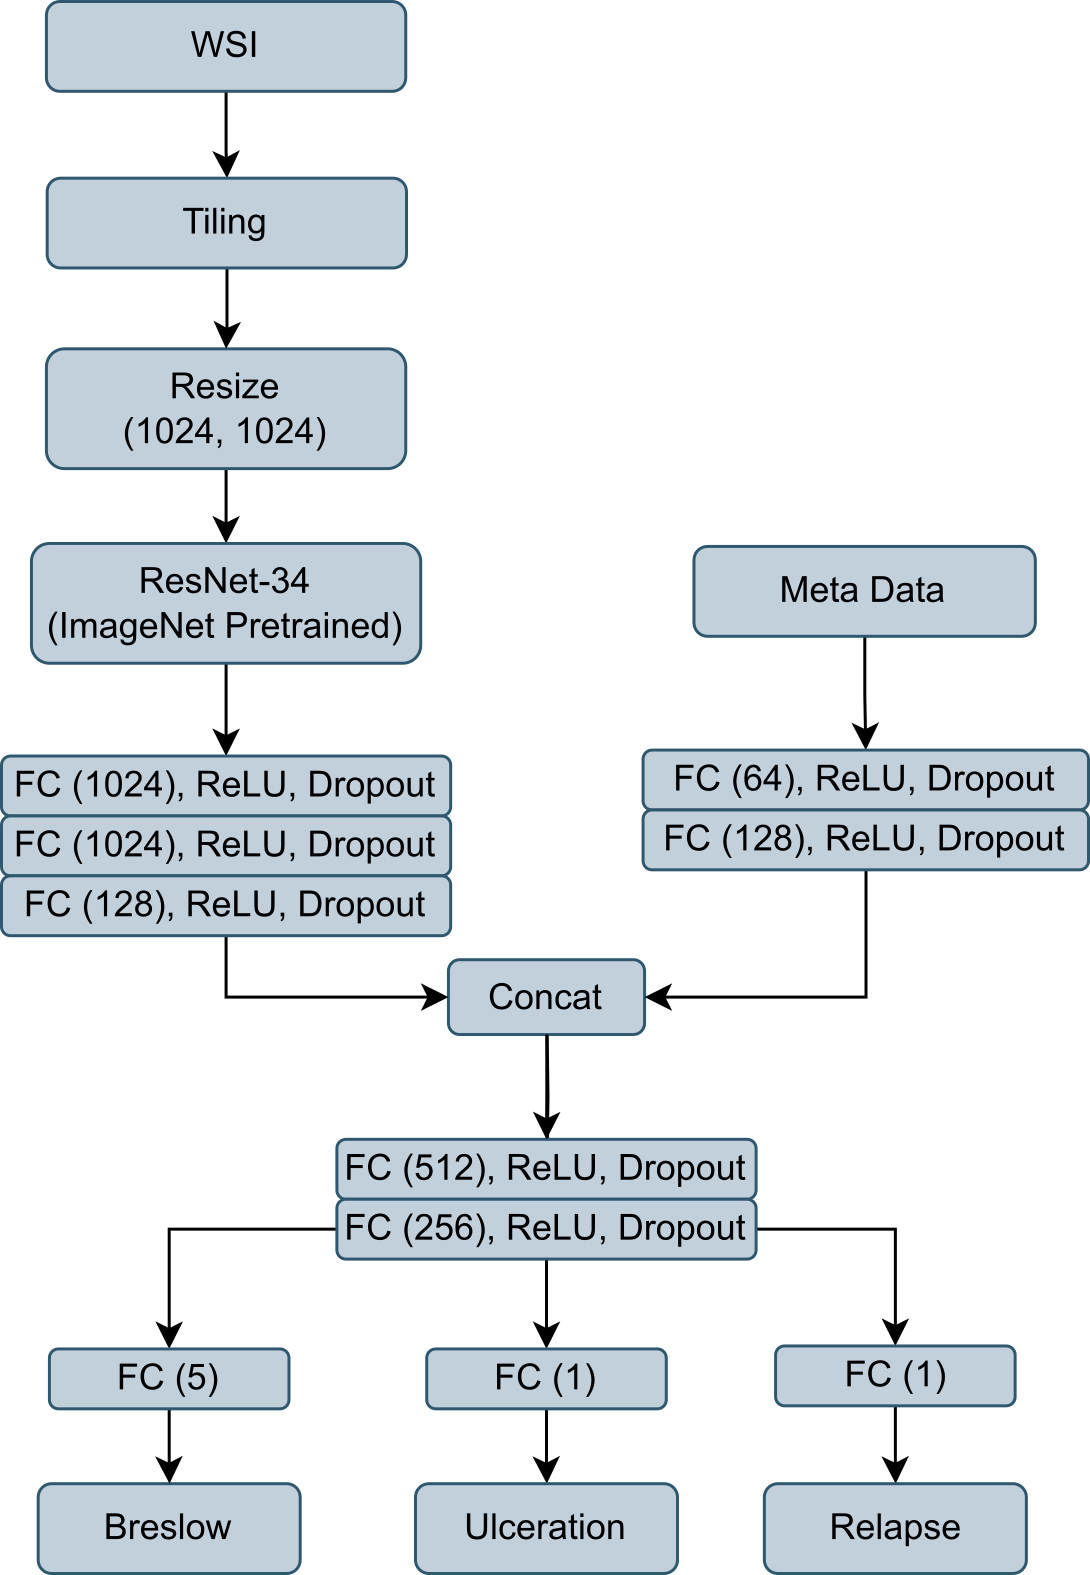
\includegraphics[scale=0.55]{images/page5.png}
  \caption{Patch Based Model Single Stage approach.}
  \label{fig:pbm_ss}
\end{figure}
\end{document}

